\documentclass[../../main]{subfiles}

\renewcommand\thesection{\arabic{section}}


\begin{document}

\section{General Workflow} \label{sec:}

Most of the workflow of TinyML is the same as typical ML workflow.
Figure \ref{fig:designFlowTinyML} depicts a simplified overview of
the entire workflow of TinyML.

\begin{figure}
    \centering
    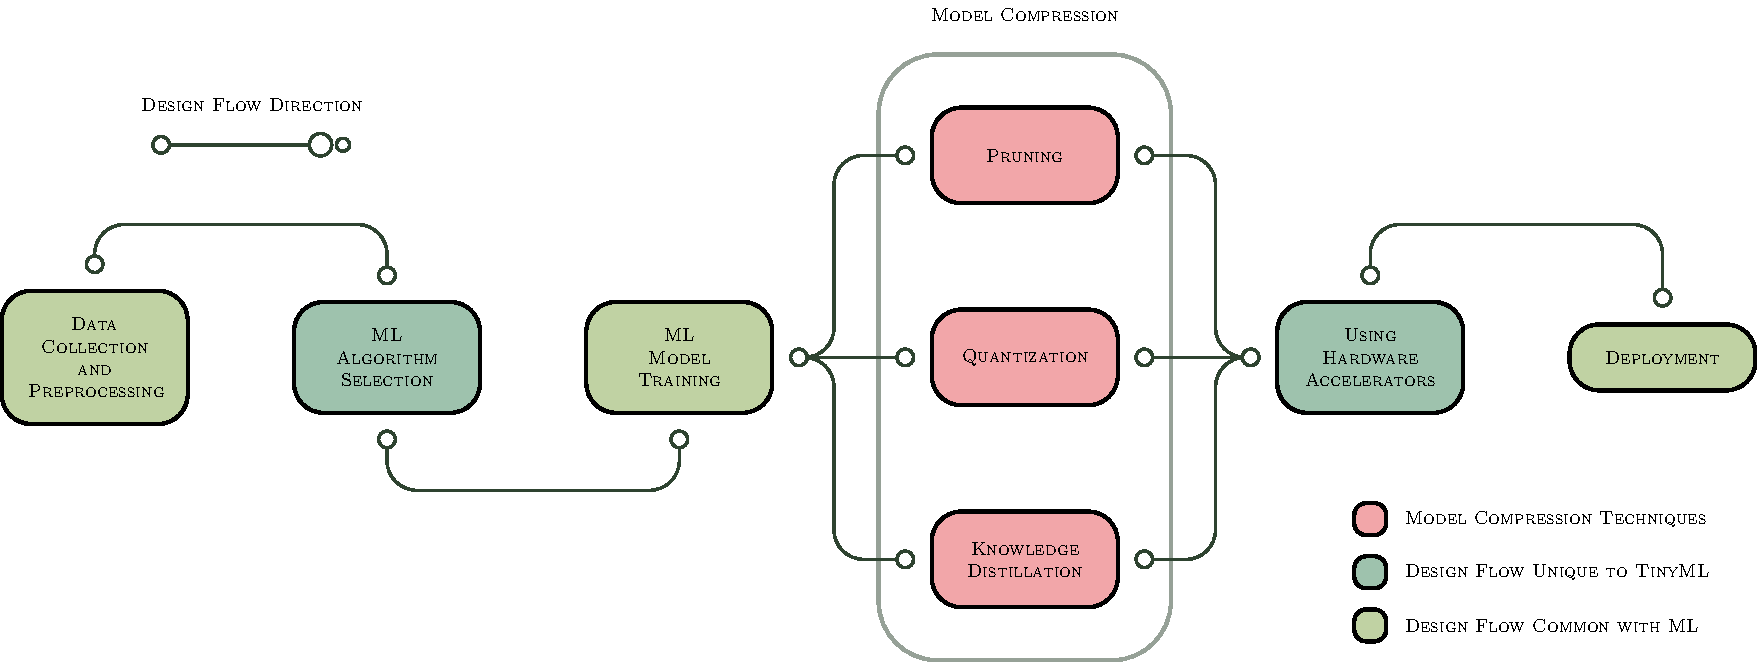
\includegraphics [
        max width = \IGXMaxWidth,
        max height = \IGXMaxHeight,
        \IGXDefaultOptionalArgs,
    ] {pics/endDesignFlow.pdf}
    \captionof{figure} {Design workflow of TinyML.}
    \label{fig:designFlowTinyML}
\end{figure}

At first we need to collect data for the training. After preprocessing we
can move on to picking an architecture\footnote{For example, MobileNet, MCUNet, etc.}.
Then we can train the model. Once we have the trained model, the core part of the
TinyML workflow comes into play, \emph{compressing} the model to fit into the
constrains of the deploying device.

Once we have a compressed model we can deploy it to the target device. In some
cases\footnote{As in the case of ESP32-S3, it has hardware AI accelerator.}, certain
devices will have hardware accelerators, so we can use them to gain more performance out
of the device.

\end{document}
